\documentclass[border=4pt]{standalone}
\usepackage{amssymb}
\usepackage{tikz}
\usetikzlibrary{arrows.meta,positioning,shapes.geometric,fit,calc,automata,trees}
\usepackage{float}
\usepackage{booktabs}
\usepackage{longtable}
\usepackage{array}
\usepackage[utf8]{inputenc}
\begin{document}

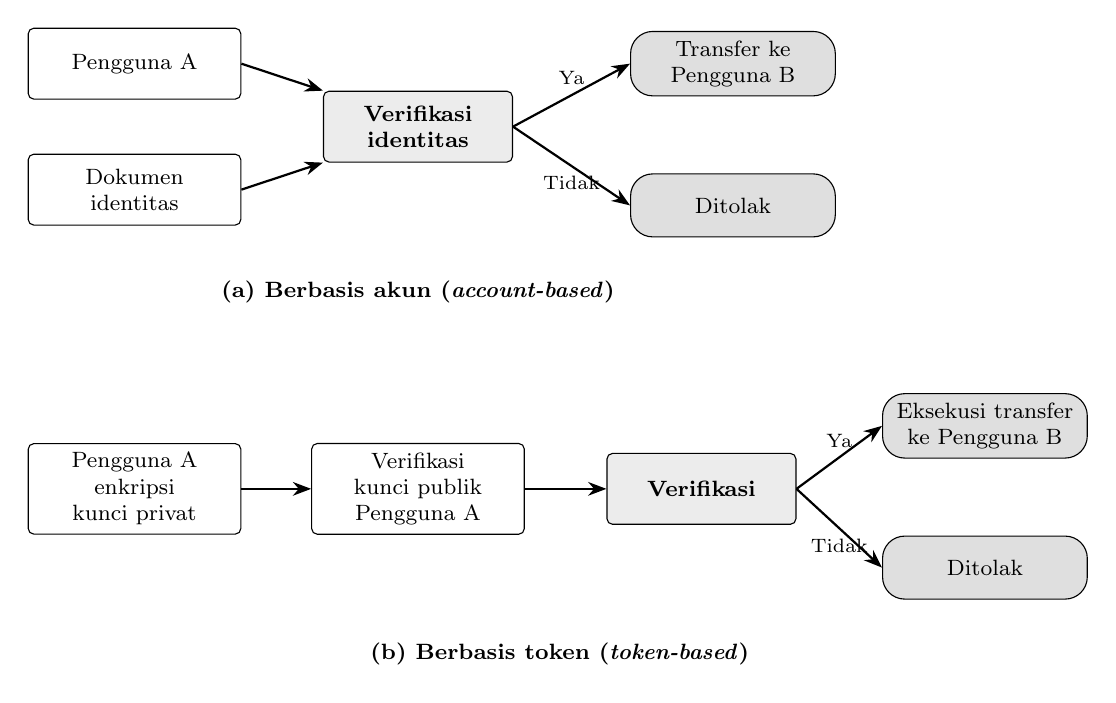
\begin{tikzpicture}[
  box/.style={draw=black, fill=white, rectangle, rounded corners=2pt,
    minimum width=2.7cm, minimum height=0.9cm, align=center, font=\footnotesize},
  ver/.style={draw=black, fill=gray!15, rectangle, rounded corners=2pt,
    minimum width=2.4cm, minimum height=0.9cm, align=center, font=\footnotesize\bfseries},
  term/.style={draw=black, fill=gray!25, rectangle, rounded corners=8pt,
    minimum width=2.6cm, minimum height=0.8cm, align=center, font=\footnotesize},
  ar/.style={-{Stealth}, thick},
]

%==== (a) Berbasis Akun ====
\node[box]  (a-user) at (0, 0.9)  {Pengguna A};
\node[box]  (a-id)   at (0, -0.7) {Dokumen\\identitas};
\node[ver]  (a-ver)  at (3.6, 0.1) {Verifikasi\\identitas};
\node[term] (a-ok)   at (7.6, 0.9) {Transfer ke\\Pengguna B};
\node[term] (a-no)   at (7.6, -0.9) {Ditolak};
\draw[ar] (a-user.east) -- (a-ver.north west);
\draw[ar] (a-id.east)   -- (a-ver.south west);
\draw[ar] (a-ver.east) -- node[above,font=\scriptsize]{Ya} (a-ok.west);
\draw[ar] (a-ver.east) -- node[below,font=\scriptsize]{Tidak} (a-no.west);
\node[font=\footnotesize\bfseries] at (3.6, -2.0)
  {(a) Berbasis akun (\textit{account-based})};

%==== (b) Berbasis Token ====
\node[box]  (b-priv) at (0, -4.5)   {Pengguna A\\enkripsi\\kunci privat};
\node[box]  (b-pub)  at (3.6, -4.5) {Verifikasi\\kunci publik\\Pengguna A};
\node[ver]  (b-ver)  at (7.2, -4.5) {Verifikasi};
\node[term] (b-ok)   at (10.8, -3.7) {Eksekusi transfer\\ke Pengguna B};
\node[term] (b-no)   at (10.8, -5.5) {Ditolak};
\draw[ar] (b-priv.east) -- (b-pub.west);
\draw[ar] (b-pub.east)  -- (b-ver.west);
\draw[ar] (b-ver.east) -- node[above,font=\scriptsize]{Ya} (b-ok.west);
\draw[ar] (b-ver.east) -- node[below,font=\scriptsize]{Tidak} (b-no.west);
\node[font=\footnotesize\bfseries] at (5.4, -6.6)
  {(b) Berbasis token (\textit{token-based})};

\end{tikzpicture}%

\end{document}
